\documentclass{article}
\usepackage[T1]{fontenc}
\usepackage{lmodern}
\usepackage{graphicx}
\usepackage{amsmath,amssymb}
\usepackage[a4paper,margin=2cm]{geometry}
\usepackage[absolute,overlay]{textpos}
\setlength{\TPHorizModule}{1mm}
\setlength{\TPVertModule}{1mm}
\usepackage[indonesian]{babel}
\usepackage{hyperref}
\setlength{\emergencystretch}{2em}
% unit: Halaman 66

\begin{document}

% === Halaman 66 (llm) ===

\section*{C. Playfair Cipher}

\begin{itemize}
    \item Ditemukan oleh Sir Charles Wheatstone namun dipromosikan oleh Baron Lyon Playfair pada tahun 1854.
\end{itemize}

\vspace{20mm}

\begin{center}
    Sir Charles Wheatstone \hfill Baron Lyon Playfair
\end{center}

% deskripsi: Foto potret Sir Charles Wheatstone
% bbox normalisasi: [0.2640, 0.4600, 0.4040, 0.7660]
\begin{textblock*}{29.40mm}(55.44mm,136.62mm)
\noindent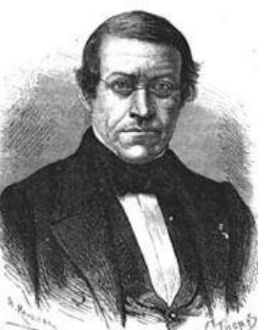
\includegraphics[width=29.40mm,height=90.88mm]{../../images/llm/page_066_img_01.png}%
\end{textblock*}

% deskripsi: Foto potret Baron Lyon Playfair
% bbox normalisasi: [0.6010, 0.4530, 0.7410, 0.7600]
\begin{textblock*}{29.40mm}(126.21mm,134.54mm)
\noindent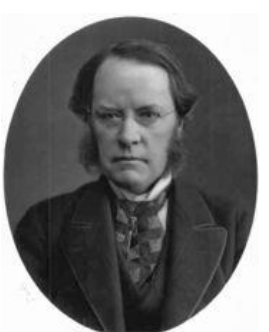
\includegraphics[width=29.40mm,height=91.18mm]{../../images/llm/page_066_img_02.png}%
\end{textblock*}

\end{document}
